
\todo[inline]{En ting å tenke på gjennom hele denne seksjonen er hvorfor du introduserer et konsept/en modell og hvem man skriver for. }

\todo[inline]{Her snakker vi om hvorfor vi introduserer tingene vi gjør. Litt om linja vi ønsker å legge oss på, den logiske oppbygningen i seksjonen etc.}

\section{Neural Networks}
The three scientific works that sparked the modern era of Neural Networks (NNs) was the proposal of the single layer Neural Network by McCulloch and Pitts in 1943 \cite{logcalc}, the first perceptron by Rosenblatt in 1958 \cite{perceptron} and the backpropagation algorithm by Werbos in 1974 \cite{backprop}.


Mathematically a Neural Network (NNs) is a function $f$ that maps an input vector $x$ to an output vector $y$ through a series of transformations. 
A NN consist of a set of interconnected nodes, or neurons, that are organized in layers. Each neuron is connected to the neurons in the previous and next layer, forming a directed graph.
To illustrate lets define a 2 layered Multilayer Perceptron (MLP) with $N$ inputs, $K$ hidden units, weights $W_1$ and $W_2$ and a single output $y$. 
\begin{figure}[H]
    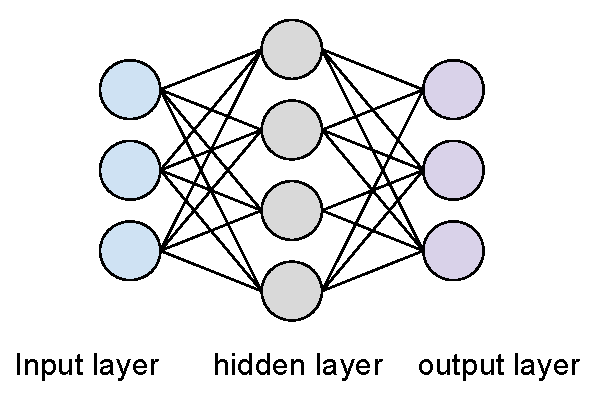
\includegraphics[scale=1]{figures/figure-pdf/NN.pdf}
    \caption{Illustration of a 2 layered MLP with $N$ inputs, $K$ hidden units, weights $W_1$ and $W_2$ and a single output $y$.}
\end{figure}

The output $y \in \R$ can be expressed as a function of the input $x\in\R^N$ and the parameters $\theta=\{ W_1 \in \R^{K \times N}, W_2 \in \R^{1\times K}, \beta \in \R^K\}$ as follows:

\begin{equation}
    y = f_\theta(x) = W_2(\sigma(W_1 x + \beta))
\end{equation}

The calculation of $y$ using the networks parameters is referd to as a feedforward operation.
The activation function, denoted as $\sigma$, determines the linearity of the output $y$. 
A concatenation of linear combinations is also a linear combination, choosing a linear $\sigma$ would result in a linear $f_\theta$.
This is not ideal, as most real world data is non-linear, meaning a straight line is not sufficient to represent the data. 
To allow the network to learn non-linear functions, non-linear activation functions are used.

Common non-linear activation functions include the sigmoid function $\sigma(x) = \frac{1}{1+e^{-x}}$ and the Rectified Linear Unit (ReLU) $\sigma(x) = \text{max}(0, x)$. 

Modern NNs build on the MLPs by adding more layers and dimensions, which is known as deep learning. The intuition being that more layers allows the network to learn more complex functions $f$ and find deeper connections between features.
A $L$-layered neural network using activation functions $\sigma^1, \sigma^2, ..., \sigma^L$, weights $W_1, W_2, ..., W_L$ and biases $\beta_1, \beta_2, ..., \beta_L$ can be expressed as follows:
\begin{equation}
    y = f_\theta(x) = \sigma^L(W_L(\sigma^{L-1}(W_{L-1}(...\sigma^1(W_1 x + \beta_1)...)+\beta_{L-1}) + \beta_L)
\end{equation}
\begin{figure}[H]
    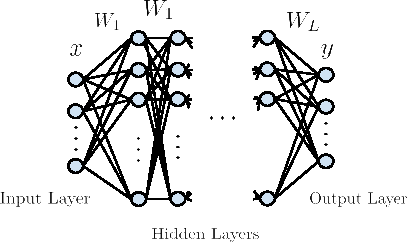
\includegraphics[scale=1]{figures/figure-pdf/NN2.pdf}
\end{figure}
\subsection{Learning in Neural Networks}
The learning process of a NN is done by adjusting the parameters $\theta$ to minimize a loss function $\mathcal{L}$. The loss function is a measure of how well the network performs on a given task.
For regression tasks the loss function is often the mean squared error (MSE) 
\begin{equation}
    \mathcal{L}_\text{MSE} = \frac{1}{N}\sum_{i=1}^N (y_i - \hat{y}_i)^2
\end{equation}
Where $y_i$ is the true value and $\hat{y}_i \in \hat{y}$ is the predicted value, $f_\theta(x) = \hat{y}$.
Learning is a optimization problem, where the goal is to find the optimal parameters $\theta^*$ that minimizes the loss function $\mathcal{L}$.
\begin{equation}
    \theta^* = \argmin_\theta \mathcal{L}
\end{equation}

The optimization is done by using the gradient of the loss function $\nabla_\theta \mathcal{L}$ to update the parameters $\theta$ in the direction of the steepest descent. This is known as gradient descent (GD).
\begin{equation}
    \theta_{t+1} = \theta_t - \alpha \nabla_\theta \mathcal{L}
\end{equation}

Where $\alpha$ is the learning rate, which determines the size of the step taken in the direction of the steepest descent. Modern NNs use the Stochastic Gradient Descent (SGD) algorithm first introduced by Herbert et al \cite{SGD} in 1951.
SGD is a variant of the GD that uses a random subset of the training data to calculate the gradient $\nabla_\theta \mathcal{L}$. This has the benefit of reducing the computational cost of calculating the gradient, as the full training set can be very large.

Gradient decent variations in addition to the technique backpropagating is typically used to train NNs. Backpropagation is a method for calculating the gradient of the loss function $\nabla_\theta \mathcal{L}$ with respect to the parameters $\theta$. Popularized in the 1980s by Rumelhart et al \cite{backprop2}.
It involves a forward pass to compute the loss, $\mathcal{L}$, and a backwards pass where the chain method is applied layer by layer, output to input, to calculate the contribution of each parameter to the total loss gradient.

These calculations require alot of computational power, which is why we have seen a surge in the use of GPUs for training NNs. GPUs are well suited for the task as they are designed to perform parallel calculations on large amounts of data. GPU technology has been a key factor in the recent success of deep learning.
Allowing larger models to be trained on larger datasets.

\section{Supervised and unsupervised learning}
Using a machine learning model there are two key learning paradigms. Supervised and unsupervised learning. Supervised learning refers to a learning process where the network has access to pre-labelled inputs which acts as targets.
For each training example there will be a set of input values alongside a designated output value. During training the model learns to mimic the labelled data by minimizing a loss function. For example the $\mathcal{L}_\text{MSE}$.

A simple example of a supervised learning task is linear regression. Here the model finds the best fit line for a given set of data points. The prediction $\hat{y}$ is determined using the equation for a line $y = ax + b$ and adjusting $a$ and $b$ to minimize $\mathcal{L}_{\text{MSE}}$.
The $\mathcal{L}_{\text{MSE}}$ requires a set of labelled data points, where the true value $y$ is known. This is the main idea behind supervised learning, and is applied to more complex models like NNs.

For a unsupervised learning the model does not have access to pre-labelled inputs. Instead the model learns to extract patterns and features from the data without any external guidance.
A example of unsupervised learning is clustering. Here the model learns to group similar data points together based on some similarity metric. Other examples include dimensionality reduction, generative models and Self Supervised Learning (SSL).

\section{Convolutional Neural Networks, CNN}

%Convolutional Neural Networks (CNNs)\cite{CNNs} is a type of neural network that is particularly well suited for processing data with a grid like topology. Examples include Images and timeseries. 
%What characterizes a CNN is the use of the convolutional operator and pooling layers.

The modern Convolutinal Neural Network (CNN) gained popularity in the 1990s, when LeChun et al\cite{LeChun} used it to classify handwritten digits. This was based on the work done by Fukushima in the 80s\cite{Fukushima} on the Neocognitron, a hierarchical, multilayered artificial neural network.
Designed to mimic the perceptive field of the the brain and the visual cortex. The Neocognitron used a convolutional operator to extract features from the input, which was then used to classify the input.
The use of a convolutional operator in Neocognitron was inspired by the work done by Hubel and Wiesel in the 60s\cite{HubelWiesel} on the visual cortex of cats and monkeys.

These works layed the foundation for modern CNNs, which are now used for a wide range of tasks including image classification, object detection, image segmentation and video analysis. 
The CNNs ability to extract features, make it well suited for data with a grid like topology. Examples include Images and timeseries. 

\subsection{Convolutional layer}
The convolutional operator is a fundamental mathematical tool that merges two functions, $x$ and $w$, to produce a third function $s$. The convolutional operator is defined as follows:
\begin{equation}
    s(t) = (x*w)(t) = \int_{-\infty}^\infty x(a)w(t-a)d a
\end{equation}
Here, $s(t)$ is the resulting function after convolution. The function $x$ is often referred to as the input, while $w$ is the filtering function also known as the kernel.
The integral runs over the entire range of $a$, combining the two values $x(a)$ and $w(t-a)$ at each point $t$ to produce $s(t)$.
As the convolutional operator is commutative, the order of the input and kernel can be swapped without changing the result.

Assuming $t$ is a integer, and using the commutative property we can express the following discrete convolution:
\begin{equation}
    S(t) = (x*w)(t) = \sum_{a=-\infty}^\infty x(a-t)w(a)
\end{equation}
Here the kernel is not dependent on the position $t$, which is beneficial in a machine learning setting because the kernel can be reused for different positions $t$. 
By defining $I$ as the input and $K$ as the kernel, we can express the discrete convolution in two dimensions:
\begin{equation}
    S(i, j) = (I*K)(i, j) = \sum_m \sum_n I(i-m, j-n)K(m, n)
\end{equation}

Here the sums calculate the dot product between the kernel, with width $m$ and height $n$, and the input at position $i, j$. This is visualized in fig \ref{fig:conv}. By calculating $S(i, j)$ for all $i, j$ we calculate the activation map $S$ corresponding to the kernel $K$ and the input $I$.
\begin{equation}
    S = \sum_i \sum_j (I*K)(i, j)
    \label{eq:activation}
\end{equation}
The activation map $S$ is a representation of the input $I$ that highlights the features detected by the kernel $K$. 
By letting $K$ have learnable parameters, the network can learn to detect features in the input through the generation of activation maps.

\begin{figure}[H]
    \centering
    \begin{center}
    \begin{figure}[H]
    \begin{tikzpicture}[
        2d-arr/.style={matrix of nodes, row sep=-\pgflinewidth, column sep=-\pgflinewidth, nodes={draw}}
      ]
    
      \matrix (mtr) [2d-arr] {
      0 & 1 & 1 & |[fill=orange!30]| 1 & |[fill=orange!30]| 0 & |[fill=orange!30]| 0 & 0\\
      0 & 0 & 1 & |[fill=orange!30]| 1 & |[fill=orange!30]| 1 & |[fill=orange!30]| 0 & 0\\
      0 & 0 & 0 & |[fill=orange!30]| 1 & |[fill=orange!30]| 1 & |[fill=orange!30]| 1 & 0\\
      0 & 0 & 0 & 1 & 1 & 0 & 0\\
      0 & 0 & 1 & 1 & 0 & 0 & 0\\
      0 & 1 & 1 & 0 & 0 & 0 & 0\\
      1 & 1 & 0 & 0 & 0 & 0 & 0\\
      };
    
      \node[below=of mtr-5-4] {$\mathbf I$};
    
      \node[right=0.2em of mtr] (str) {$*$};
    
      \matrix (K) [2d-arr, right=0.2em of str, nodes={draw, fill=teal!30}] {
        1 & 0 & 1 \\
        0 & 1 & 0 \\
        1 & 0 & 1 \\
      };
      \node[below=of K-3-2] {$\mathbf K$};
    
      \node[right=0.2em of K] (eq) {$=$};
    
      \matrix (ret) [2d-arr, right=0.2em of eq] {
      1 & 4 & 3 & |[fill=blue!80!black!30]| 4 & 1\\
      1 & 2 & 4 & 3 & 3\\
      1 & 2 & 3 & 4 & 1\\
      1 & 3 & 3 & 1 & 1\\
      3 & 3 & 1 & 1 & 0\\
      };
      \node[below=of ret-4-3] {$\mathbf{I * K}$};
    
      \draw[dashed, teal] (mtr-1-6.north east) -- (K-1-1.north west);
      \draw[dashed, teal] (mtr-3-6.south east) -- (K-3-1.south west);
    
      \draw[dashed, blue!80!black] (K-1-3.north east) -- (ret-1-4.north west);
      \draw[dashed, blue!80!black] (K-3-3.south east) -- (ret-1-4.south west);
    
      \foreach \i in {1,2,3} {
          \foreach \j in {4,5,6} {
              \node[font=\tiny, scale=0.6, shift={(-1.2ex,-2ex)}] at (mtr-\i-\j) {$\times \pgfmathparse{int(mod(\i+\j,2))}\pgfmathresult$};
            }
        }
    \end{tikzpicture}
    \caption{Example of convolutional operation. $\mathbf{I}$ is the input, $\mathbf{K}$ is the kernel and $\mathbf{I} * \mathbf{K}$ is the activation map. Illustration taken from the Random TikZ collection\cite{RiebesellTikZ2022}}
    \end{figure}
    \end{center}
    
    \caption{Example of convolutional operation. $\mathbf{I}$ is the input, $\mathbf{K}$ is the kernel and $\mathbf{I} * \mathbf{K}$ is the activation map. Illustration taken from the Random TikZ collection\cite{RiebesellTikZ2022}}
    \label{fig:conv}
\end{figure}

The configuration of a convolutional layer involves not only the selection of the kernel size ($m$, $n$) but also the specification of the stride length and the padding. 
The stride defines the number of units the filter shifts over the input data for each convolution operation. A stride of 1 implies the $i,j$ gets incremented by 1 in eq \ref{eq:activation}.
This makes for a more fine-grained $S$ compared to a stride of 2, which would increment $i,j$ by 2 for each calculation. The use of a higher stride reduces the dimensionality of the output $S$.
Which is beneficial when the task is to compress the input into a smaller activation map.

\subsection{Pooling and Downsampling}
A pooling layer, also refered to as a detector stage, is a component of CNNs that reduces the dimensionality of the input data.
It works as a downsampler, reducing the spatial size of the input data by applying a filter. The filter is applied to a region of the input, and the output is a summary of the region.

The most common pooling operations are:
\begin{itemize}
    \item \textbf{Max Pooling:} Selects the maximum element from the region of the feature map covered by the filter. This method is effective at capturing the presence of features.
    \item \textbf{Average Pooling:} Computes the average of the elements in the region of the feature map covered by the filter, which helps in smooth feature representation.
\end{itemize}

\begin{center}
    \begin{figure}[H]
    \begin{tikzpicture}[
        2d-arr/.style={
            matrix of nodes,
            nodes in empty cells,
            row sep=-\pgflinewidth,
            column sep=-\pgflinewidth,
            nodes={minimum size=1cm, draw, anchor=center, scale=0.7}
        },
        pool-box/.style={
            draw=red, thick, rounded corners
        },
        scale = 0.7
    ]

    \matrix (input) [2d-arr] {
         2 & 1 & |[fill=orange!30]| 3 & 0 \\
        |[fill=orange!30]| 4 &  3 & 2 &  1 \\
        0 & 2 & 1 & |[fill=orange!30]| 4 \\
        |[fill=orange!30]| 3 & 2 &  1 & 1 \\
    };

    \node[left=of input-2-1.west, anchor=center, rotate=90] {Input Feature Map};
    
    \matrix (output) [2d-arr, right=2cm of input] {
        |[fill=blue!30]| 4 & |[fill=blue!30]| 3 \\
        |[fill=blue!30]| 3 & |[fill=blue!30]| 4 \\
    };

    \node[right=of output-2-2.east, anchor=center, rotate=90] {Max Pooled Feature Map};

    \draw[pool-box] (input-1-1.north west) rectangle (input-2-2.south east);
    \draw[pool-box] (input-1-3.north west) rectangle (input-2-4.south east);
    \draw[pool-box] (input-3-1.north west) rectangle (input-4-2.south east);
    \draw[pool-box] (input-3-3.north west) rectangle (input-4-4.south east);

    \draw[->, thick] (input) -- (output) node[midway, above] {Max Pooling};

    \end{tikzpicture}
\caption{Illustration of a max pooling operation. The input feature map is reduced in size by applying a max pooling filter with size 2x2 (red boxes), which selects the maximum value in each filter region to produce the max pooled feature map.}
\end{figure}
\end{center}

Using a pooling layer in the context of CNNs help summarize the activation map $S$ and reduce the dimensionality. This helps to mitigate overfitting aswell as reducing the computational cost of the network.

\subsection{Architecture of CNNs}
A typical CNN architecture consists of the following layers:

\begin{itemize}
    \item \textbf{Convolutional Layer} — Applies the learnable filters on the input data, producing a activation map. Each filter detects different features by convolving with the input.
    \item \textbf{Activation Function} — Typically, a ReLU is applied to introduce non-linearity into the model, allowing it to learn more complex functions.
    \item \textbf{Pooling} — This layer reduces the spatial size of the representation, reducing the number of parameters and computation in the network, and hence, also controlling overfitting. 
    \item \textbf{Fully Connected Layer} — Neurons in a fully connected layer have full connections to all activations in the previous layer. Primarely used for processing the information obtained through the convolutional layers to perform a task like classification.
\end{itemize}


\section{Residual block}
The residual block, pioneered by He et al. in their paper on deep residual learning \cite{ResLearn}, represents a advancement in neural network arcitecture, 
specifically addressing the challenges of training deeper networks.

The problem at hand, as described by He et al, is that deeper networks are more difficult to train. This challenge is primarily attributed to the vanishing gradient problem.
In deeper networks, the gradient of the loss function tends to diminish progressively, complicating the training process. 
This emerges from the key mechanism in the backpropagation algorithm, the chain rule. The chain rule, a mathmatical principle, decomposes the gradient computation into a series of smaller,
more manageable calculations. In deeper networks this recursive procedure can lead to increasingly smaller gradient values due to accumulating errors in the large amount of smaller calculations. 

The residual block, visualized in fig \ref{fig:resblock}, introduces a arhitecture feature known as the "shortcut connection" that helps mitigate this issue.
Mathematically, if we consider the standard layer operation as a function $F(x)$, where $x$ is the input to the layer, the output of a typical layer would be just $F(x)$. In the residual block,
we define the output to be $H(x) = F(x) + x$. This addition of $x$ is the shortcut connection. Its a form of identity mapping ensuring that the deeper layers can, at the very least, achieve the performance of shallower
networks by simply learning the identity function for the additional layers.

\begin{figure}[H]
    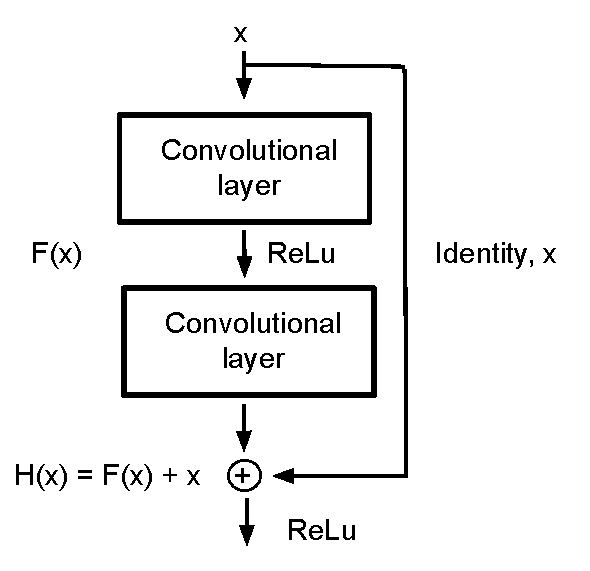
\includegraphics[scale=0.6]{figures/figure-pdf/Resnet.pdf}
    \caption{Illustration of the Resnet block from He et al's original paper\cite{ResLearn} }
    \label{fig:resblock}
\end{figure}

\section{Self Supervised Learning, SSL}
Self-supervised learning (SSL) is a form of unsupervised learning where the data itself provides the supervision. SSL algorithms learn to predict unobserved or hidden parts of the input from observed parts.
This is achieved trough carefully designed loss functions, which enforce the learning of usefull features by solving pretext tasks. Modern mainstream SSL frameworks can be divided into two categories, contrastive and non-contrastive learning.

\subsection{Contrastive and Non Contrastive learning}
Contrastive learning is a popular method in SSL, particularly for learning visual representations. It relies on contrasting positive pairs (similar or related data points) against negative pairs (dissimilar or unrelated data points). 
The intuition is to learn embeddings such that similar samples are closer to each other in the embedding space, while dissimilar ones are farther apart. Take the example of dogs and cats,
a contrastive approach would seperate the dog embeddings from the cat embeddings. Several prominent contrastive learning methods, such as MoCo\cite{MoCo} and SimCLR\cite{SimCLR}, effectively utilize positive and negative pairs to learn contrasted representations.

Non-Contrastive learning methods in SSL, by contrast, does not depend on negative pairs. Instead, these approaches aim to learn representations by encouraging similarity between different augmented views of the same data point. 
This approach is based on the principle that different transformations of the same data should yield similar representations, thereby ensuring consistency and robustness in the learned features.
Augmented versions of the same cat, should yield the same cat embedding. Notable non-contrastive methods include BYOL (Bootstrap Your Own Latent)\cite{BYOL} and Barlow Twins \cite{Barlow}.

\subsection{The Role of Siamese Networks in SSL}
Siamese networks\cite{Siamese} is a neural network architecture designed for specialized tasks that require the comparison of input pairs. The defining characteristics of these networks is the dual-branch structure, where two identical sub-networks with shared parameters process two seperate inputs.
The outputs of the sub networks, often refered to as twin embeddings, are then brought togheter to evaluate the degree of similarity or difference. The similarity or difference is then used to calculate a contrastive or non contrastive loss function.
The siamese architecture is illustrated in fig \ref{fig:Siamese}. 

\begin{figure}[H]
    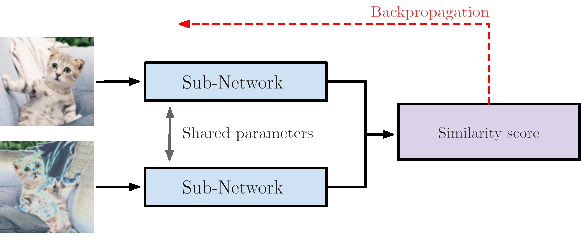
\includegraphics[scale=1]{figures/figure-pdf/Siamese.pdf}
    \caption{ Example of a non contrastive siamese network using augmented views. Here the images are processed to calculate a similarity score, the backpropagation arrow indicates that the similarity score is then used to update the weights of the sub network. Pictures taken from \url{www.pexels.com}}
    \label{fig:Siamese}
\end{figure}


Many modern SSL approaches base their architecture on the siamese network as it is efficient for teaching a sub network to discriminate between different classes or features in a dataset. 


\subsection{Barlow Twins}
The Barlow Twins method, introduced by Zbontar et al in their 2021 article "Self-Supervised Learning via Redundancy Reduction"\cite{Barlow}, presents a alternative non-contrastive objective function for SSL. The core idea being an objective function that encourages the learning of feature representations
by reducing redundancy while retaining critical information from the input data. 

The rationale behind the objective function, $\mathcal{L}_{\text{BT}}$, is grounded in the properties of the identidy matrix. Viewing the identity matrix as a cross correlation matrix the zero valued off diagonal elements indicates no redundancy between different features. Since the diagonal elements are ones it suggest that each feature is similar, containing similar informational value.
Thereby, if a cross correleation matrix equals the identity matrix we have achieved no redundancy and full informative value between the features.

\subsubsection{Objective function of Barlow Twins}
The objective function, or similarity score, of the Barlow Twins method can be formulized as follows:

\begin{equation}
\mathcal{L}_{BT}(\mathbf{z_1}, \mathbf{z_2}) = \sum_i (1 - C_{ii})^2 + \lambda \sum_i \sum_{j \neq i} C_{ij}^2
\end{equation}

where $C$ is the cross correlation matrix computed between the outputs ($\mathbf{z_1}$ and $\mathbf{z_2}$) of two identical networks fed with distorted version of the same data (siamese style). $C_{ii}$ is the diagonal elements and $C_{ij}$ is the offdiagonal elements.
The parameter $\lambda$ controls the trade-off between invariance and redundancy reduction.

\subsubsection{Siamese architecture}
The barlow Twins method builds apon the siamese architecture, where each subnetwork consists of a encoder and a projector.

The procedure is as follows. First a batch normalization is applied to the distorted views ($x_A$, $x_B$), allowing the data to be normalized before being fed into the encoder, $E$.
Typically $E$ is implemented using convolutional layers and residual blocks that create non linear activation maps with reduced dimensions, capturing the essense of the data. The latent variables are then fed into the projector, $P$.
The projector, $P$, acts as a dimensionality expander with learnable parameters. Typically a deep fully connected neural network. It learns to expand the encodings into a space where the barlow twins loss can be efficiently applied.
The intuition behind expanding the dimensions is that more features in the cross-correlation matrix enable a more efficient and robust comparison while also allowing the model to capture a broader range of characteristics within the encodings.
Next the empirical cross correlation is compared with the Identity matrix as visualized in fig \ref{fig:Barlow}

\begin{figure}[H]
    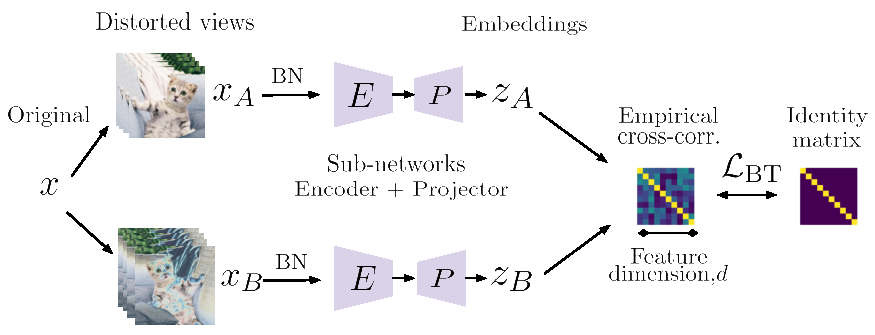
\includegraphics[scale=0.8]{figures/figure-pdf/BarlowT.pdf}
    \caption{Illustration of the Barlow Twins procedure, inspired by the original paper\cite{Barlow}.}
    \label{fig:Barlow}
\end{figure}

The optimalization problem is then to minimize the objective function $\mathcal{L}_{BT}$ with respect to the parameters of the encoder and projector. The result is parameters that produce encodings that are invariant to distortions while also being informative.
Typical appliances includes using the encoder as a feature extractor for tasks like classification.

\section{The Vector Quantized Variational Autoencoder, VQ-VAE}
The Variational Autoencoder first introduced by Kingma and Welling in 2013\cite{VAE} is a probabilistic model that learns the underlying distribution of the input data, which can then be used to generate new data points. It is a type of autoencoder, which is a neural network designed to learn
representations of the input in a unsupervised manner. First introduces in the 1980s by Rumelhart et al\cite{Rumelhart}. The Vector Quantized Variational Autoencoder (VQVAE), introduced by van den Oord et al\cite{neuvqvae} in 2017, is a variant of the VAE that uses discrete latent variables instead of continuous ones.
This discretization of the latent space has shown to be a evolutionairy step from the VAE, improving the representations and quality of the generated data.

\subsection{Evolution from Variational Auto-Encoder, VAE}
As a fundemental principle of latent variable models, the Autoencoder explicates the relationship between the observed data and latent variables (unobserved) through the marginal distribution. This relationship is central to understanding how a autoencoder encodes and decodes data, capturing the essence of the data's underlying structure.

Lets consider a dataset, denoted as $\mathbf{x}=\{x_1, x_2, \cdots, x_n \}$, which comprises observed data points. Corresponding to these data points, we have latent variables $\mathbf{z}=\{z_1, z_2, \cdots, z_n \}$, which represent hidden factors or features extracted by the autoencoder.
The model parameters denoted as $\theta$, govern the transformation from data to latent space and vice versa.

The bayesian relationship is explained by the marginal distribution, expressed as follows:

\begin{equation}
    p_\theta(x) = \int_zp_\theta(x, z) dz= \int_z p_\theta(z)p_\theta(x|z)dz    
\end{equation}
\subsubsection{Variational inference and optimization}
The optimization problem is to optimize $\theta$ to efficiently transform input data into a latent representation and reconstruct the input based on the latent representation.
Using the posterior $p_\theta(\mathbf{x}|\mathbf{z})$ and prior $p_\theta(\mathbf{z})$. All parameterized by $\theta$.
\subsubsection{Challenges in Maximum Likelihood Estimation}
Optimizing the model parameters \( \theta \) through Maximum Likelihood Estimation poses significant computational challenges. The optimization objective for \( \theta \) is to maximize the log likelihood of the observed data:

\begin{equation}
    \theta^* = \argmax_\theta \sum_{i=1}^n \log p(x_i | \theta)
\end{equation}

However, this requires evaluating an integral over the latent distribution that is intractable:

\begin{equation}
    \theta^* = \argmax_\theta \sum_{i=1}^n \log\int_{z_i}p_\theta(x|z)p_\theta(z)
\end{equation}

\subsubsection{Variational Approximation}
To circumvent the intractability of the integral, we approximate the posterior \( p_\theta(z|x) \) with an encoder model \( q_\phi(z|x) \), parameterized by a neural network with variational parameters $\phi$, that maps the input data to the latent space.
Hence giving the autoencoder the name Variational Autoencoder (VAE). The decoder neural network aims to reconstruct the input data $\mathbf{x}$, thereby approximating the conditional likelihood $p_\theta(\mathbf{x}|\mathbf{z})$.

\begin{equation}
    \mathbf{x}\rightarrow \underset{\sim q_\phi(\mathbf{z}|\mathbf{x})}{\text{EncoderNeuralNet}_\phi(\mathbf{x})} \rightarrow \mathbf{z} \rightarrow \underset{\sim p_\theta(\mathbf{x}|\mathbf{z})}{\text{DecoderNeuralNet}_\theta(\mathbf{z})} \rightarrow \hat{\mathbf{x}}
\end{equation}

\subsubsection{Evidence Lower Bound}
Due to the infeasibility of optimizing the likelihood directly it becomes necessary to adopt an alternative objective function. This function incorporates the variational aproximated posterior, $q_\phi(\mathbf{z}|\mathbf{x})$, and is commonly known as the Evidence Lower Bound (ELBO), denoted as $\mathcal{L}_{\theta, \phi}(x)$.

\begin{equation}
    \mathcal{L}_{\theta, \phi}(x) = \log p_\theta(x) - \mathcal{D}_{KL}(q_\phi(z|x) || p_\theta(z|x))
    \label{eq:ELBO}
\end{equation}

The first term in the ELBO, $\log p_\theta(x)$, represents the log likelihood of the data under the model parameters $\theta$. This term encourages the reconstructed data $\hat{\mathbf{x}}$, generated by the decoder network, to be as close as possible to the original input data $\mathbf{x}$.
The second term, 
\begin{equation}
\mathcal{D}_{KL}(q_\phi(z|x) || p_\theta(z|x))
\end{equation}
is the Kullback-Leibler (KL) divergence between the approximate posterior distribution $q_\phi(\mathbf{z}|\mathbf{x})$ and the true underlying distribution, $p_\theta(\mathbf{z}|\mathbf{x})$.

By maximizing the ELBO with respect to \( \theta \) and \( \phi \) we achieve the following:

\begin{enumerate}
    \item Enhancement of the marginal likelihood \( p_\theta(x) \), leading to improved reconstruction of the input data by the decoder.
    \item Reduction of the Kullback-Leibler (KL) divergence between the approximate posterior \( q_\phi(z|x) \) and the true posterior \( p_\theta(z|x) \), resulting in a more accurate encoder model for the latent variables.
\end{enumerate}

By maximizing the ELBO, we get a two for one, we refine the model's parameters to enhance data reconstruction accuracy and improve the encoder's inference of the latent representations, aligning them more closely with the true assumed underlying distribution.\cite{VAE}
\subsection{Transition to discrete latent variables}
VQ-VAE retains the encoder-decoder structure but introduces a discrete twist. It employs a vector quantization mechanism that translates the continuous latent variables of a traditional VAE into discrete ones, denoted as $\mathbf{z_q}$

The fundamental shift from continous to discrete latent variables influences the dynamics of the model. In a VAE, the priors and posteriors are typically assumed gaussian. This assumption enables the application of the reparameterization trick\cite{1312.6114}, which is beneficial for effective training, primarily due to its contribution to
reducing gradient variance. However its important to note that this approach imposes a constraint that both the prior and posterior must conform to the underlying assumption of its shapes. This requirement, while beneficial for certain aspects of training, introduces a limitation in the models flexibility to represent a wider variety of data distributions.


\subsubsection{Vector quantization}
Vector quantization (VQ) is a key component of the VQ-VAE model, first proposed by van den Oord et al\cite{neuvqvae}. Within the architecture of the VQ-VAE, the encoder transforms input data into a series of continuous latent vectors. These vectors are then discretized through vector quantization,
which maps each continuous vector to the closest embedding vector in a predefined set known as the codebook.

The codebook, denoted by $\Zstroke$, is composed of $K$ discrete embedding vectors (or tokens), expressed as $\Zstroke = \{z_k\}_{k=1}^K$. Here $K$ represents the cardinality of the discrete latent space,
implying that the latent space comprises K distinct categories. Each embedding vector $z_k$ resides in a $d$-dimensional space. $z_k \in \R^d$

Quantization is implemented through a nearest neighbor search within $\Zstroke$. For any given continuous latent vector $z_{ij}$, the quantized vector $(z_q)_{ij}$ is determined by locating the token $z_k \in \Zstroke$ that minimizes the euclidian distance to $z_{ij}$.

$$(z_q)_{ij} = \argmin_{z_k \in \Zstroke}|| z_{ij} - z_k ||$$

\subsubsection{Effect on KL divergence}
As Van den Oord et al describes in their paper \cite{neuvqvae} each latent vector index maps deterministically to a single embedding vector in the codebook. As a result, the probability distribution of the latent indices given any input is a one-hot distribution. 
This means that for any given input, the posterior assigns a probability of one to a single latent index and zero to all others. 
\begin{equation}
    q(z = z_q | x) =
    \begin{cases}
    1 & \text{if } q = \argmin_{z_q \in \Zstroke} || z_{ij} - z_q || \\
    0 & \text{otherwise}
    \end{cases}
\end{equation}
(Stemmer formuleringen her??)

We can investigate the effects on the KL divergence by viewing the model as a VAE, as Van den Oord in his paper. Meaning that we bound $\log p_\theta(x)$ by the ELBO $\mathcal{L}_{\theta, \phi}$.
By now defining a simple uniform distribution over $z$ and using the one-hot deterministic $q(z=z_q|x)$ we can derive the KL-divergence as follows

\begin{equation}
    \begin{aligned}
        \mathcal{D}_{KL}(q_\phi(z|x) || p_\theta(z)) &= \sum_i q(z=q|x) \log \frac{ q(z=q|x)}{p(z=q)} \\
        &= \log K
    \end{aligned}
\end{equation}
(Skriv om .. Noen bruker p(z) andre p(z|x) for Kullback. Brukte p(z|x) i ELBO)

The constant KL divergence indicates a stable relationship between the aproximate posterior and the prior. The relationship is stable regardless of any assumption of shapes and forms for the posterior. This efficiently
addresses the "posterior collapse" or "KL vanishing"\cite{posteriorcollapse} issue commonly encountered in traditional VAEs. Posterior collapse occurs when the latent variables become less informative as the decoder learns to ignore the information provided by the 
encoder. In VQVAE, by allowing the posterior to take any shape without being bound by the constraints of a Gaussian distribution, the model maintains significance of the latent variables throughout training. 
